%preamble
\documentclass[letterpaper]{article}
\synctex=1
\usepackage{graphicx}
% \graphicspath{ {images/} }

% \usepackage{lipsum}
\usepackage{float}

%actual document
\begin{document}
\begin{figure}[H]
    \centering
    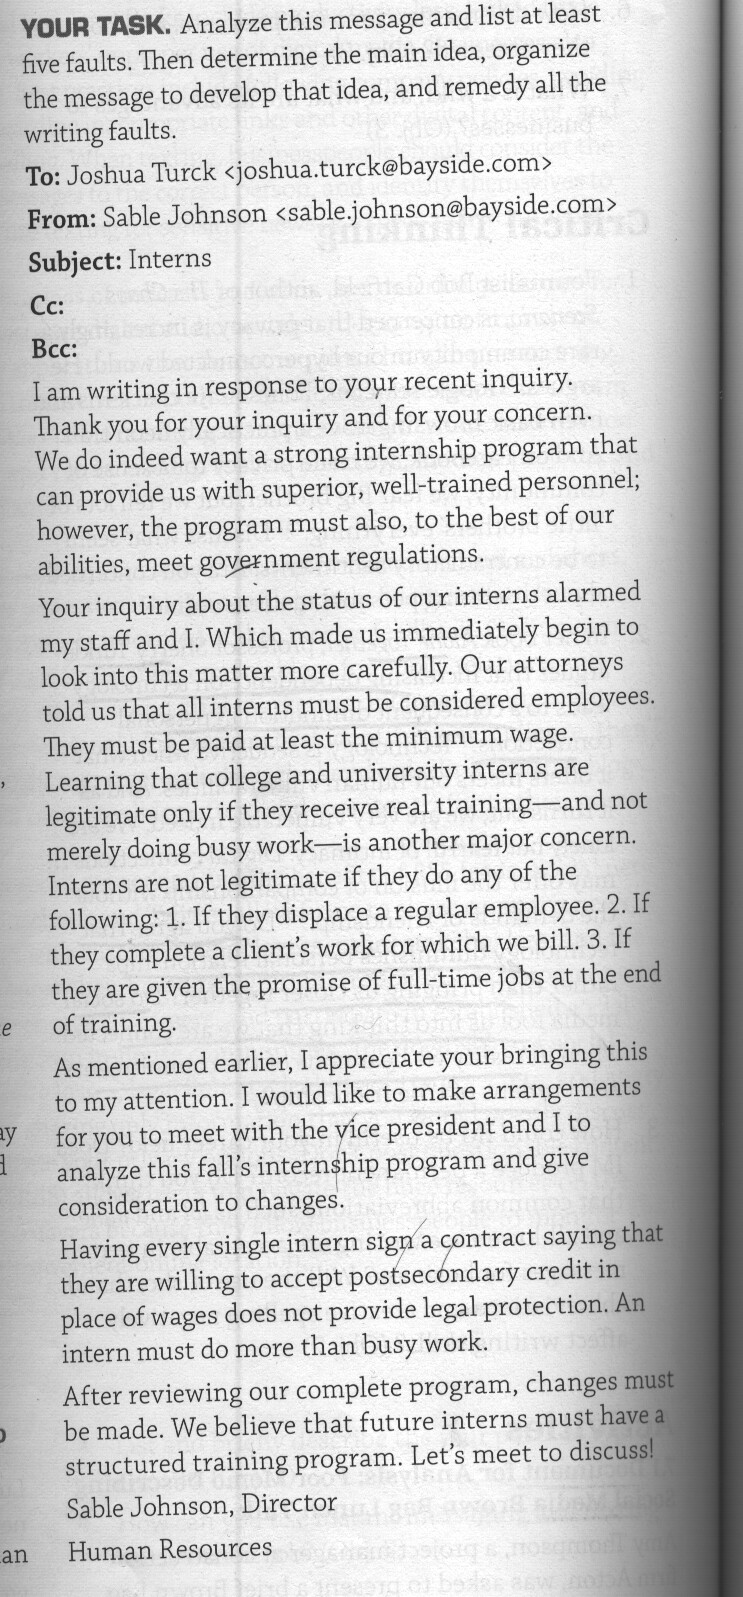
\includegraphics[\textwidth]{EffectiveWritingWorkshop.jpg}
    \caption{Original picture}
\end{figure}



Thank you for your inquiry and for your concern. While we want a
strong internship program that can provide us with superior, well-trained
personel, our proram should also meet government regulations.

Your inquiry about the status of our interns alarmed my staff and I, which made us
immediately begin to look into this matter more carefully. Our attorneys
have told us that all interns must be considered employees.
As employees, they must be paid at least the minimum wage.
Another major concern is that college and university interns
are legitimate only if they receive real training as opposed to
doing busy work.
Interns are not legitimate if they do any of the following:
\begin{enumerate}
  \item They displace an employee
  \item They compete a client's work for which we bill
  \item They are given the promise of full-time jobs at the end of training
\end{enumerate}

\par
I appreciate you bringing this to my attention. I would like to make
arrangements for you to met with the vice president and I to analyze
this fall's internship program and give consideration to changes.

Having every single intern sign a contract saying that they are willing
to accept postsecondary credir in place of wages does not provide
legal protection, because an intern must do a busy woork.


Changes should be made after reviewing our complete program. We believe that future
interns must have a structured training program.

\vspace{1cm}
Sable Johnson, Director

\vspace{.5cm}
Human Resources
\end{document}
